% !TeX root = ../Thesis.tex

%************************************************
\chapter{Evaluation}\label{ch:evaluation}
%************************************************
\glsresetall % Resets all acronyms to not used

We perform both quantitative and qualitative evaluation to assess how well our implementation fulfills the requirements we set ourselves in \cref{ch:introduction}. This allows for a comprehensive judgement of what future development of \gls{HiPS} should focus on.

\section{Recommended settings}
\label{sec:recommendedSettings}
For our evaluation to be exhaustive, we would have to test a plethora of available hardware and software configurations. Since this is not feasible, we focus on entry-level smartphones and recommended settings. Thereby, we assume the lowest common denominator in hardware. We expect this to give us a good estimate of how useful our app would be in the real world. Both quantitative and qualitative evaluation is done on the smartphones listed in \cref{tab:smartphones} earlier, using our \gls{LLM} of choice, Llama 3.2 1B.

Similarly, we focus on running the steganography algorithms with our recommended settings: For Arithmetic coding, we recommend \lstinline|temperature| = 1.0, \lstinline|topK| = 128,256 tokens (the \gls{LLM}'s vocabulary size) and \lstinline|precision| = $ \lceil \log_2(topK) \rceil $ = 17 bits. This is based on the results of Stegasuras, which showed that Arithmetic coding can achieve the optimum of no \gls{KL} divergence with an unmodulated \gls{LLM}~\cite{zieglerNeuralLinguisticSteganography2019}. For Huffman coding, we recommend \lstinline|bitsPerToken| = 2 bits/token. This is because in our subjective judgement, it offers the best trade-off between cover text quality and length. Quality is similar to \lstinline|bitsPerToken| = 1 at twice the efficiency, making cover texts 50\% shorter. With \lstinline|bitsPerToken| = 3, quality degrades significantly, starting diminishing returns for savings in length. Arithmetic compression is recommended in any case. Lastly, we recommend the context length to be 2 messages. This is because in our subjective judgement, cover text quality was sufficient while computational costs can nearly be minimized with this setting.

\section{Quantitative evaluation}
\label{sec:quantitativeEvaluation}
Quantitative evaluation of our app focusses on three dimensions: Performance, efficiency and reliability. We measure performance as the speed of token generation, efficiency as the ratio of Arithmetic compression over UTF-8, and reliability as the success rate of cover text decoding. All three are crucial factors for gaining acceptance amongst users.

\subsection{Performance}
\label{sec:performance}
To appeal to a large user base, we set ourselves the requirement of acceptable performance on entry-level devices. We measure performance via the speed of token generation, as this is the main task of our app. \cref{tab:performance} shows the encoding and decoding speeds we achieved for every combination of smartphone and algorithm. The speeds were averaged over a conversation of ten cover texts, each encoding a random sentence of up to five words as secret message. With both of our entry-level devices measuring at around 1 token/second, user experience is smooth enough to fulfill our requirement.

\begin{table}
	\centering
	\begin{tabular}{@{} lrr @{}} % @{} removes white spaces
		\toprule
		\tableheadline{Device} & \tableheadline{Encoding} & \tableheadline{Decoding} \\
		\midrule
        Arithmetic               &                 &                 \\
		\midrule
        Moto One Vision          & $1.24 \pm 0.21$ & $1.26 \pm 0.21$ \\
		Moto E13                 & $0.95 \pm 0.11$ & $0.95 \pm 0.11$ \\
        Samsung Galaxy S24 Ultra & $3.59 \pm 0.40$ & $3.54 \pm 0.38$ \\
        \midrule
        Huffman                  &                 &                 \\
        \midrule
        Moto One Vision          & $1.24 \pm 0.15$ & $1.26 \pm 0.17$ \\
		Moto E13                 & $0.92 \pm 0.08$ & $0.92 \pm 0.09$ \\
        Samsung Galaxy S24 Ultra & $3.44 \pm 0.49$ & $3.27 \pm 0.50$ \\
		\bottomrule
	\end{tabular}
	% Use alternative short title for table of contents
	\caption[Performance measurements]{Average encoding and decoding speeds and their standard deviations for every combination of smartphone and algorithm. All values are measured in tokens/second.}
	\label{tab:performance}
\end{table}

However, our implementation shows a considerable performance deficit in comparison to other apps running \glspl{LLM} with llama.cpp: In \cref{sec:howToRunLLMsOnAndroid}, we found that we can achieve around to 5 tokens/second on the same smartphones. Overhead is similar on our flagship device, which achieved up to 4 tokens/second with our app versus up to 25 tokens/second with the other apps. This is likely because the other implementations we investigated perform token sampling in C++ rather than Kotlin. Therefore, they don't have to pass data through the \gls{JNI} for every token. We underestimated the impact of this design decision in the early phases of development due to lack of experience.

\subsection{Corrupted cover texts}
\label{sec:corruptedCoverTexts}
Due to the probabilistic nature of \glspl{LLM}, the responses they generate are hard to predict. But as \glspl{LLM} are stateless, their responses to a given prompt should be reproducible (see \cref{sec:tokenGenerationWithLlamaCpp} for details). In particular, this should apply to the cover text tokens generated during steganographic encoding and decoding. In our testing, we encountered some issues with this. While the vast majority of cover texts could be decoded, some were corrupted: For these cover texts, the token predictions of the \gls{LLM} were inconsistent between encoding and decoding. This renders the encoded secret messages unrecoverable.

To quantify this, we generated ten conversations of ten cover texts. Each cover text encoded a random sentence of up to five words as secret message. Each conversation was given a different system prompt. We did this for both algorithms, using the recommended settings defined earlier. Arithmetic coding was able to decode 98 out of the 100 cover texts, Huffman coding achieved 97 out of 100.

While this is robust enough for a demonstration, it should be investigated further to make \gls{HiPS} ready for production. Stegasuras already mentions that this issue may be related to the use of tokenization based on \gls{BPE}~\cite{zieglerStegasuras2025}. While Stegasuras already implements some fixes~\cite{zieglerHarvardnlpNeuralSteganography2025}, translating them to our implementation could not resolve the issue reliably. Future research may also investigate how significant this is when using larger, less quantized \glspl{LLM}, as those supposedly are more accurate. Users can however already bypass the issue in most cases by simply sending an affected secret message again, so that it gets encoded it with a different context.

\section{Qualitative evaluation}
\label{sec:qualitativeEvaluation}
While our implementation of steganography is based on the Stegasuras project~\cite{zieglerNeuralLinguisticSteganography2019}, our approach for steganalysis differs. We evaluate robustness of our cover texts against human eavesdroppers via a survey.

\subsection{Survey design}
\label{sec:surveyDesign}
Stegasuras performed steganalysis by asking humans if a given sentence was a plausible continuation of a context taken from a news article~\cite{zieglerNeuralLinguisticSteganography2019}. While such an approach would allow us to calculate a success rate for fooling humans with our cover texts, its applicability is limited. Stegasuras already mentions that a head-to-head comparison of two possible continuations of the same context is uncommon in everyday life~\cite{zieglerNeuralLinguisticSteganography2019}. Our use case of creating chat conversations from cover texts introduces further limitations. While the plausibility of news articles can be judged by their factual accuracy~\cite{zieglerNeuralLinguisticSteganography2019}, chat messages often don't contain objectively verifiable claims. Instead, they regularly contain personal information that is only verifiable by the people chatting with each other.

Therefore, we chose to evaluate to what extent our cover texts fulfill certain linguistic characteristics typically found in chat messages. A study among Canadian university students serves as a framework~\cite{alazzawieLinguisticSituationalFeatures2022}, as the audience for our survey is expected to be similar (i.e. students of TU Darmstadt). We summarize the characteristics found in this framework as follows: Use of correct grammar/spelling, use of emojis, and use of abbreviations. As these characteristics can easily be influenced via the system prompt, we expect this approach to give us insights in how to refine it further. We added the length of chat messages as a new characteristic. This helps us understand how significant the compression overhead of our implementation is. We use a 5-point Likert scale~\cite{likertTechniqueMeasurementAttitudes1932} for each of the four characteristics. As Likert scales are a widely used method for gathering user feedback in software development, we expect participants to quickly be familiar with them~\cite{girayAssessmentStudentSatisfaction2021,tizardVoiceUsersExtended2022}.

We presented participants of our survey with screenshots of six chat conversations: Four were cover texts generated by the \gls{LLM} (two for each algorithm), two were real (donated by members of the SEEMOO group). We generated cover texts by encoding random sentences of up to five words with system prompts similar to the example shown earlier in \cref{fig:lmStudio}. \cref{ch:survey} contains all chat conversations we used, both real and cover texts, and the system prompts corresponding to the cover texts. We asked participants to rate how similar these conversations are to their own messages using the Likert scales (e.g. "I use emojis in a similar way" from 1 = "Strongly disagree" to 5 = "Strongly agree"). We also gave them the option to add comments to explain their ratings for each conversation. Participants did not know any of the conversations were generated by a \gls{LLM}, as we presented the survey to be about linguistics rather than steganography.

\subsection{Survey results}
\label{sec:surveyResults}
Our survey delivered valuable insights in how to increase cover text quality further. \cref{fig:likertplots} shows an overview of the results. Most of the 31 participants rated the real conversations as more similar to their own chats than the cover texts. Cover texts were rated the most dissimilar in the use of emojis. This is explained in the comments ten participants gave: The \gls{LLM} tends to use emojis rather mechanically. For example, "I'm running late" may be followed by a clock emoji. Instead of enriching cover texts with non-verbal communication by expressing emotions, this only reiterates what is already being said.

\begin{figure}
    \begin{wide}
        \centering
        \captionsetup{width=\linewidth}
        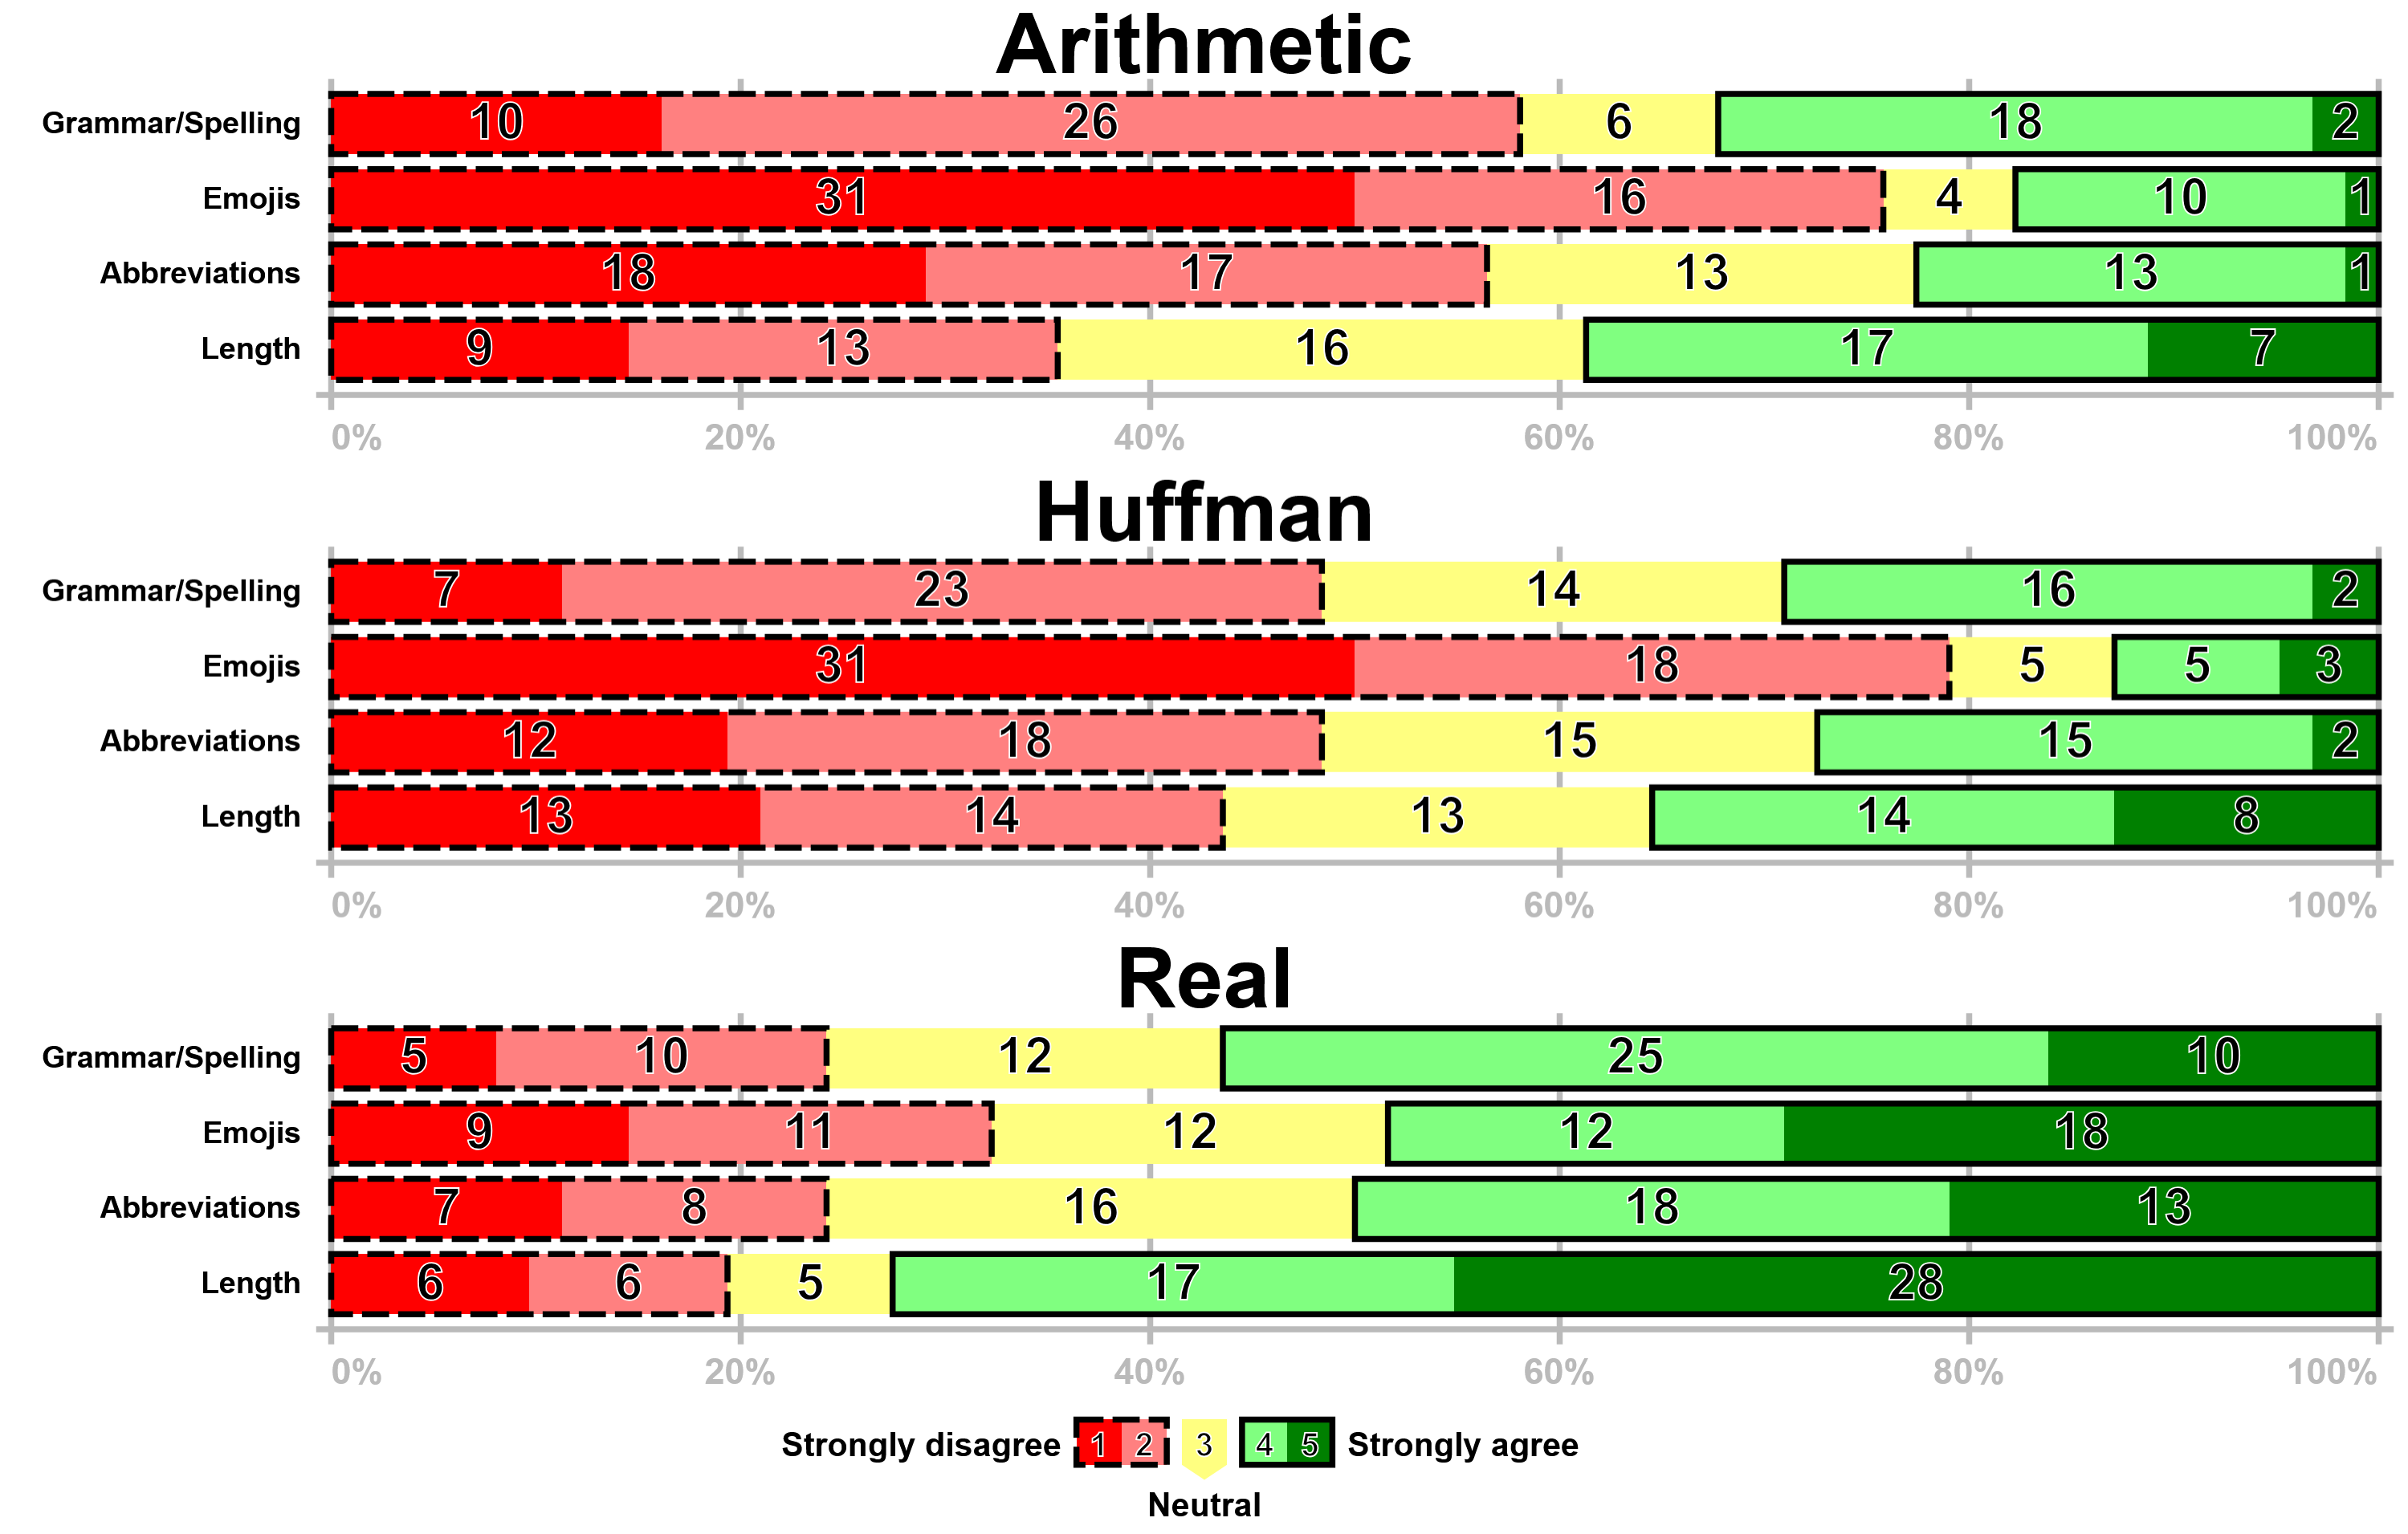
\includegraphics[width=\linewidth]{likertplots.png}
        \caption[Survey: Results]{Survey results. Similarity ratings on the Likert scales are aggregated for cover texts from Arithmetic coding, cover texts from Huffman coding, and real messages, respectively. Created using~\cite{maurerLikertplotcomPlotLikert2013}.}
        \label{fig:likertplots}
    \end{wide}
\end{figure}

Higher similarity was achieved in the use of grammar/spelling and abbreviations. Participants expressed various personal preferences regarding the use of specific emojis and abbreviations. Furthermore, four participants commented that they don't include interjections or sounds (e.g. "oh", "ugh") in their messages, which the \gls{LLM} tends to do. Training a \gls{LLM} on one's own chat messages as demonstrated in~\cite{donnerSimulationMeFinetuning2024} may therefore be promising. Message length was rated the most similar. This implies that users of our app would have to restrict themselves to secret messages of around five words to generate plausible cover texts.

Overall, this survey highlights the variety with which chat messages reflect our personalities. Anecdotally, seven participants commented that they write messages similar to our cover texts, while two other participants commented that the same cover texts look like they were generated by a \gls{LLM}. One participant commented that our cover texts were typical for older people, who may write more formal messages like pen pals, as opposed to younger people, who may be more chaotic in their communication. As our participants were mostly students of TU Darmstadt, they belong to a relatively young demographic. This may have introduced a bias in our survey. The study we use as framework supports this by suggesting that there may be two kinds of users, divided by writing more functional versus more elaborate messages~\cite{alazzawieLinguisticSituationalFeatures2022}. Repeating this survey while targeting an older demographic could therefore be promising.

\subsection{Demographic limitations and randomization}
\label{sec:demographicLimitationsAndRandomization}
With 31 participants, our survey is not representative. It is specific to our choice of \gls{LLM}, system prompts, recommended settings and demographic of participants. The latter still needs to be discussed. In addition to rating linguistic characteristics, we asked participants for their age range and native language. All participants were German-speakers in the two youngest age ranges (18-24 and 25-34), which is to be expected with students of TU Darmstadt. Due to the limited ability of small \glspl{LLM} to speak languages other than English, we presented participants with both English cover texts and real messages. We deem this acceptable as our participants have an academic background.

Lastly, randomization is limited further by the small number of conversations. This is due to the lack of publicly available datasets of organic chat messages. Some public datasets from instant messengers like WhatsApp exist~\cite{ueberwasserWhatsSwitzerlandCorpusbased2017}, but they rarely contain messages in German. We did not use datasets from adjacent fields (e.g. Reddit comments~\cite{baumgartnerPushshiftRedditDataset2020} or Telegram channels~\cite{morgiaTGDatasetCollectingExploring2025}), as these mostly don't follow the dialogue structure typical for instant messaging.
